\documentclass{article}

\usepackage[T1]{fontenc}    %Schriftart des Dokumentes
\usepackage[ngerman]{babel} %Dokumentensprache, hier Deutsch
\usepackage{amsmath, amssymb, stmaryrd} %mathematische Schriftzeichen
\usepackage{graphicx} %Einfügen von Grafiken
\usepackage{wrapfig}
\usepackage{bm}

\setlength{\parindent}{0pt} %Einrückung von Absätzen auf null gesetzt
\setlength{\parskip}{10pt} %Abstand zischen Absätzen auf 10pt gesetzt

\title{Versuch 34: Spektralphotometrie}
\author{Matthias Kuntz}
\date{08.09.2023}

\begin{document}

\maketitle

\addtocounter{figure}{2}

%-------------------------EINLEITUNG-------------------------
\section{Einleitung}

In diesem Versuch soll mithilfe der Spektralphotometrie der Extinktionskoeffizient einer Kaliumpermanganatlösung (KMnO$_4$) bei Licht einer Wellenlänge von $\lambda = 525nm$ ermittelt werden. Hierzu wird die Absorption vom Licht zunächst als Funktion der Schichtdicke, dann als Funktion der Konzentration der Lösung betrachtet.

\subsection{Physikalische Grundlagen}

Grundlage dieses Versuchs ist die Fotometrie, die Konzentrationsbestimmung einer Substanz durch Absorption. Beginnend mit der Messung der Abschwächung der Lichtinsität eines einfallendes Lichtbündels, ausgelöst durch die in der Messzelle enthaltene Substanz, kann über das Absorptionsgesetz folgender Zusammenhalt hergestellt werden:

\begin{equation}
    \begin{split}
        \frac{dI}{I} &= -kdl \\
        \implies I &= I_0 e^{-kl} \ \ \ \ \ \text{(Lambertsches Absorptionsgesetz)}
    \end{split}
\end{equation}

Dabei sind $I_0$ die in das Medium eindringende Lichtintensität, $k$ die Absorptionskonstante und $l$ die Länge des Lichtwegs. Bei unserer Auswertung wird halblogarithmisches Papier verwendet, weshalb die logarithmische Schreibweise mit dekadischem Logarithmus relevant ist:

\begin{equation}
\begin{split}
    \ln{I} &= -kl + \text{const} \ \ \ \text{mit} \ \ \ \text{const} = \ln{I_0} \\
    \log_{10}{I} &= -k'l + \text{const'} \ \ \ \text{mit} \ \ \ k' = \log_{10}{(e)} \ k 
\end{split}
\end{equation}

Wobei $k'$ dekadischer oder Bunsenscher Absorptionskoeffizient genannt wird.

Für verdünnte Lösungen mit gegebener Konzentration $c$ [$\frac{mol}{l}$ oder $\frac{mol}{cm^3}$] gilt das Beersche Gesetz:

\begin{equation}
    k' = \epsilon c
\end{equation}

$\epsilon$ wird molarer Extinktionskoeffizient oder Molarextinktion genannt und ist eine von $c$ unabhängige Stoffkonstante. Hierbei können bei höheren Konzentrationen Abweichungen vom Beerschen Gesetz auftreten. 

Werden die beiden Gesetze aus Gleichungen 2 und 3 kombiniert so erhält man:

\begin{equation}
    I = I_0 10^{-\epsilon c l}
\end{equation}

Somit ist die Intensität im Allgemeinen sowohl abhängig von der Konzentration als auch von der Schichtdicke der Lösung. 

Ein wichtiger Bestandteil dieses Versuchs ist ein Gitterspektrometer. Bei diesem wird der einfallende Lichtstrahl zunächst über eine Lichtleitfaser in das Spektrometer eingekoppelt und über Umleitungen mit Spiegeln zunächst von einem optischen Gitter reflektiert, welches das Licht wellenlängenabhängig reflektiert und es somit aufspaltet, und mithilfe einer Linse auf eine CCD-Zeile mit Lichtsensoren abgebildet. Somit entsteht das digitale Signal, welches von der zugehörigen Datenerfassungssoftware dargestellt werden kann. In der Software können dann Modifizierungen wie die Eliminierung des Hintergrundlichts vorgenommen werden.

\subsection{Versuchsaufbau}

Eine Skizze des Versuchsaufbaus ist in Abbildung 3 zu sehen. Die Lichtquelle strahlt hier Licht mit der Ausgangsintensität durch einen Spalt und eine Linse auf die in der Küvettenbank angebrachten Küvetten, die die absorbierende Lösung enthalten. Danach wird das Licht über den Fasereinkoppler zum Gitterspektrometer und schließlich von dort digital zum Computer geleitet.

Zunächst werden bei konstanter Konzentration Küvetten mit verschiedener Länge auf der Küvettenbank angebracht und die Intensität bei festgehaltener Wellenlänge untersucht. Daraufhin wird die Schichtdicke konstant gehalten und es wird untersucht, wie sich die Intensität bei zunehmender Konzentration der Lösung in der Küvette verändert.

\newpage

\begin{figure} [h]
    \centering
    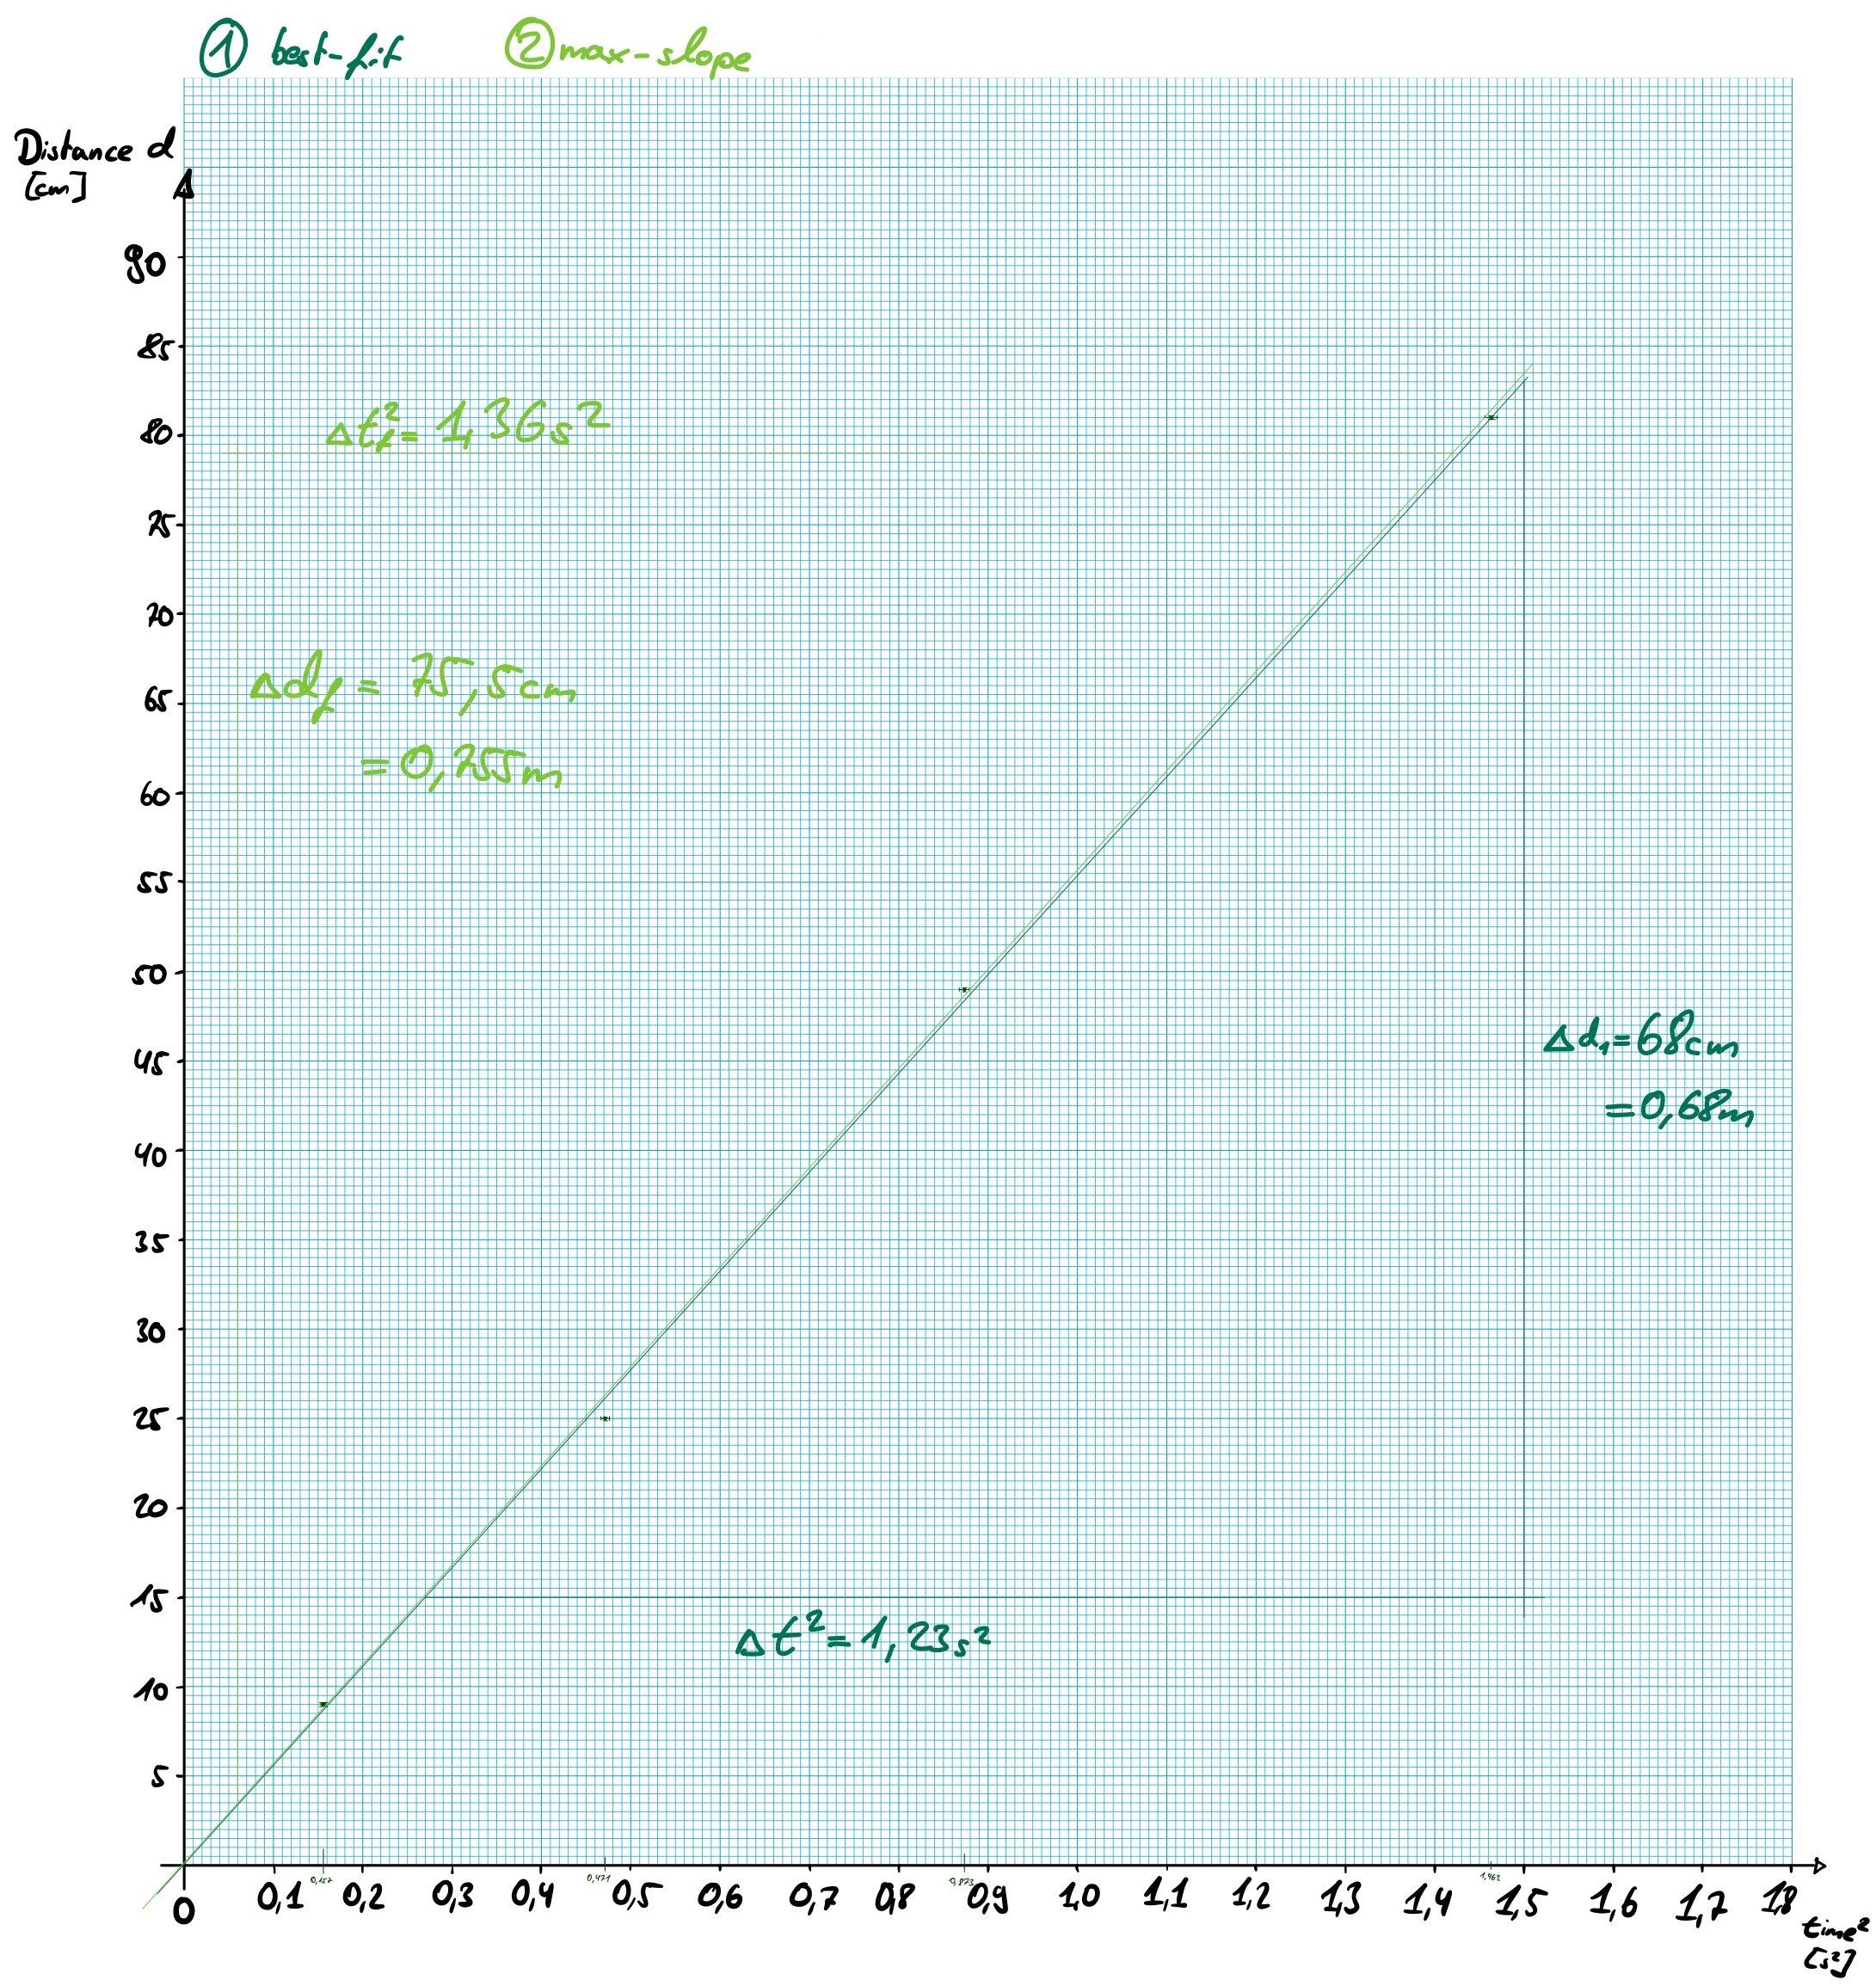
\includegraphics[width=\textwidth]{graphics/dia1.jpg}
    \caption{Skizze des Versuchsaufbaus}
\end{figure}

\newpage

%---------------VERSUCHSPROTOKOLL MIT MESSDATEN---------------
\newpage

\section{Versuchsprotokoll mit Messdaten}

\includegraphics[width=\textwidth]{graphics/mess1.jpg}
\newpage
\includegraphics[height=\textwidth, angle=90]{graphics/mess2.jpg}
\newpage
\includegraphics[width=\textwidth]{graphics/mess3.jpg}
\newpage
\includegraphics[width=\textwidth]{graphics/mess4.jpg}
\newpage
\includegraphics[width=\textwidth]{graphics/mess5.jpg}
\newpage

\addtocounter{table}{3}

%-------------------------AUSWERTUNG-------------------------
\section{Auswertung}

\subsection{Zu Aufgabe 2}

Zunächst werden die Ergebnisse aus Tabelle 1 in ein Diagramm auf halblogarithmischem Netzpapier eingetragen, zu sehen in Abbildung 2 im Messprotokoll. Dabei wird auf der Abszisse die Küvettenlänge und auf der Ordinate die Intensität abgebildet. Man bestimmt die Steigung der Ausgleichsgeraden $m_1$ und die der Fehlergeraden $m_{f_1}$ mithilfe der eingezeichneten Steigungsdreicke.

Es wird zuerst mit Gleichung 2 der Extinkionskoeffizient $k'_1$ und dessen Fehler $\Delta k'_1$ über die Differenz von $k'_1$ und $m_{f_1}$ bestimmt:

\begin{equation}
    \begin{split}
        k'_1 &= m_1 = \frac{\Delta I_1}{\Delta l} = 0,1089 \frac{1}{cm} \\
        \Delta k'_1 &= \left| k'_1 - m_{f_1} \right| = \left| k'_1 - \frac{\Delta I_{f_1}}{\Delta l_{f}} \right| = 0,0006 \frac{1}{cm}
    \end{split}
\end{equation}

Mit Gleichung 3 wird nun die Molarextinktion $\epsilon_1$ und deren Fehler $\Delta \epsilon_1$ mit dem Fehlerfortpflanzungsgesetz bestimmt. Man verwendet $c = 5 \cdot 10^{-5} \frac{mol}{l}$:

\begin{equation}
    \begin{split}
        \epsilon_1 &= \frac{k'_1}{c} = 2178 \frac{l}{mol \cdot cm} = 2178000 \frac{cm^2}{mol} \\
        \Delta \epsilon_1 &= \sqrt{\left( \frac{\Delta k'_1}{{c}} \right)^2} = 12 \frac{l}{mol \cdot cm} = 12000 \frac{cm^2}{mol}
    \end{split}
\end{equation}

\subsection{Zu Aufgabe 3}

Analog zu Aufgabe 2 verläuft hier die Berechnung. Zunächst werden aus dem Diagramm die Steigung der Beer-Geraden $m_2$ und die der zugehörigen Fehlergeraden $m_{f_2}$ bestimmt.

Somit erhält man zunächst für den Extinktionskoeffizienten:

\begin{equation}
    \begin{split}
        k'_2 &= m_2 = \frac{\Delta I_2}{\Delta c} = 2699,2 \frac{l}{mol} \\
        \Delta k'_2 &= \left| k'_2 - \frac{\Delta I_{f_2}}{\Delta c_f} \right| = 114,0 \frac{l}{mol}
    \end{split}
\end{equation}

Und für die die Molarextinktion:

\begin{equation}
    \begin{split}
        \epsilon_2 &= \frac{k'_2}{l} = 1799 \frac{l}{mol \cdot cm} = 1799000 \frac{cm^2}{mol} \\
        \Delta \epsilon_2 &= \sqrt{\left( \frac{\Delta k'_2}{l} \right)^2} = 76 \frac{l}{mol \cdot cm} = 76000 \frac{cm^2}{mol}
    \end{split}
\end{equation}

\subsection{Vergleich der Ergebnisse}

Zuletzt werden die bestimmten Werte für $\epsilon_1$ und $\epsilon_2$ miteinander verglichen. Dazu wird die Sigmaabweichung berechnet. Es gilt:

\begin{equation}
    \sigma = \frac{\left| \epsilon_1 - \epsilon_2 \right|}{\sqrt{(\Delta \epsilon_1)^2 + (\Delta \epsilon_2)^2}} = 4,93
\end{equation}

Was somit auffallend hoch ist.

\newpage
%---------------PRÄSENTATION DER ENDERGEBNISSE---------------
\section{Präsentation der Endergebnisse}

Bei diesem Versuch wurde auf zwei verschiedenen Wegen die Molarextinktion mit Licht einer Wellenlänge von 525nm durch Variatrion von Schichtlänge und Konzentration einer KMnO$_4$-Lösung bestimmt. Es wurden folgende Werte bestimmt:

\begin{equation}
    \begin{split}
        \bm{\epsilon_1} &= \bm{2178 \pm 12 \frac{l}{mol \cdot cm}} \\
        \bm{\epsilon_2} &= \bm{1799 \pm 76 \frac{l}{mol \cdot cm}} \\ \\
        \iff \bm{\epsilon_1} &= \bm{2178000 \pm 12000 \frac{cm^2}{mol}} \\
        \bm{\epsilon_2} &= \bm{1799000 \pm 76000 \frac{cm^2}{mol}}
    \end{split}
\end{equation}

\newpage
%---------------ZUSAMMENFASSUNG UND DISKUSSION---------------
\section{Zusammenfassung und Diskussion}

In diesem Versuch wurde auf zwei verschiedene Weisen die Molarextinktion einer Kaliumpermanganatlösung bestimmt, indem durch Spektralphotometrie die Intensität eines Lichtstrahls nach Durchlaufen desser mit einem Gitterspektrometer digital bestimmt wurde. Bei ersten Versuchsteil wurde die Länge der zu durchlaufenden Küvetten variiert und beim zweiten die Konzentration der Lösung, startend bei reinem Wasser bis hin zu einem Mischung, die zur Hälfte Wasser und zur anderen Hälfte Kaliumpermanganat war. Anschließend wurde mithilfe des Ampereschen und Beerschen Gesetzes zunächst der Extinktionskoeffizient und dann die Molarextinktion grafisch bestimmt.

Bezüglich potenzieller Fehlerquellen lässt sich anmerken, dass die digitale Bestimmung der Intensitäten mit dem Computer den Ablesefehler praktisch komplett eliminiert, solange das Programm vorher richtig konfiguriert und dann richtig verwendet wurde. Zudem kommt dazu, dass beim ersten Versuch die Küvettenlängen alle gegeben exakt waren, weshalb hier auch kein Fehler entstand. 

Etwas anders sieht das schon beim zweiten Versuchsteil aus. Da hier die Konzentration der Lösung selbst abgefüllt werden musste, liegt hierbei eine hohe potenzielle Fehlerquelle. Die Skalen an den Flüssigkeitsbehältern waren zwar recht genau, jedoch waren das Abfüllen selbst als auch das darauffolgende Vermischen der Flüssigkeiten sicherlich fehlerbelastet. 

Zudem kommt die allgemeine Fehlerbelastung der grafischen Methode. Bei uns fällte während dem Zeichen besonders auf, dass die einzelnen Werte keine Gerade auf dem logarithmischen Papier bildeten, wodurch das Zeichnen der Ausgleichsgerade schwierig abzuschätzen war. Zudem kommt, dass die berechneten Fehler vor allem in den ersten Werten immer viel zu klein waren, um sie sinnvoll in das Diagramm einzuzeichnen, weshalb auch die Bestimmung der Fehlergeraden recht mühsam war. Auch ist das Ablesen aus dem Diagramm sicherlich nicht zwangsläufig perfekt. 

Aufgrund dieser Fehlerquellen entstand dann auch unser Ergebnis mit einer Sigmaabweichung von $\sigma = 4,93$. Diese Abweichung ist sogar so groß, dass sich die Frage nach systematischen Fehlern stellt. 

Ideen hierzu wären zum einen das Alter von den Küvetten verschiedener Längen sowie potenzielle Fehler der Angaben des Programms. Bei Ersterem ließen sich nämlich Aufkleber auf den Küvetten finden, die diese auf das Jahr 1984 datierten. Zwar ist mir nicht klar, inwiefern solche Küvetten altersanfällig sind, jedoch wirkt es insbesondere bei so einem gravierend abweichenden Ergebnis wie bei uns doch schonmal erwähnenswert. Über Fehler des Programms kann ich natürlich keine genaueren Vermutungen anstellen, jedoch würde beispielsweise schon eine leicht fehlerhafte Dunkelmessung ein anderes Ergebnis liefern. Eine weitere Tatsache ist, dass wir den Fehler des Strahlengangs durch lange Küvetten nur bei der letzten berücksichtigt haben, was die Werte der anderen auch leicht beeinflussen wird. 

Systematische Fehler speziell beim zweiten Versuch ließen sich nur in der abgefüllten Lösung finden. Eine leicht vom angegebenen $\Tilde{c}$ abweichende Konzentration oder ein systematischer Abfüllfehler unserer Seite wären denkbar. 

Allgemein lässt sich noch anmerken, dass der Versuchsaufbau von uns nicht aufgebaut oder modifiziert wurde, sondern bereits einsatzbereit vor Ort war. Somit sind potenzielle Fehler bei der Einstellung der Objekte auf der Schiene oder Konfigurationen der einzelnen Bauteile nicht ausgeschlossen, können aber somit auch nicht von uns bewertet werden.  

Insgesamt lässt sich aber dennoch das erste Verfahren als genauer bewerten, da hier einfach mehr Angaben von vornherein gegeben waren und sich unsere Interaktion mit dem Versuchsaufbau auf das Einlegen der Küvette auf die Schiene sowie das Ablesen einer Zahl auf dem Bildschirm beschränkte. 

Zum Schluss lässt sich das Fazit ziehen, dass bei diesem Versuch leider kein aussagekräftiges, verlässliches Ergebnis erzielt werden konnte, dafür ist die Abweichung der beiden bestimmten Werte einfach zu groß. Dafür konnte eine intensivere kritische Auseinandersetzung mit den beiden Methoden erfolgen, was die Abschätzung der genaueren Methode interessanter machte. 

\end{document}

